% GENERATED by assemble.py from front.tex, back.tex and ../algorithm/main.tex. Edit those, not this file.
% AIAA student-conference paper, combined version: the impossibility result and the landing algorithm in one paper
% (11-page limit). Standalone: cites neither of the two separate papers. Shared format: ../aiaa-format.tex.
% Source files: front.tex (this file), back.tex, and sections taken from ../algorithm/main.tex by assemble.py.
% Build: python3 assemble.py && latexmk -pdf main.tex   (from this directory)
% Shared format for the two AIAA student-conference papers in this folder (impossibility/ and algorithm/).
% AIAA Meeting Paper (conference) format, reproduced from the published instructions
% ("Preparation of Papers for AIAA Technical Conferences"): letter paper, 1 in margins, Times 10 pt, single column,
% single spaced; title bold 24 pt; abstract bold, indented 0.5 in each side; section headings bold 11 pt, centered,
% Roman numerals; subsections bold flush left with capital letters; sub-subsections italic with arabic numerals;
% captions bold ("Fig. 1" below figures, "Table 1" above tables); footnote symbols; numbered references.
% To use AIAA's own class instead, replace everything between the two "FORMAT" markers by
%     \documentclass[conf]{new-aiaa}  plus the packages and macros marked KEEP,
% and move the title, authors and abstract into that class's \title, \author, \affil and abstract commands.
% ----------------------------------------------------------------------------------------------- FORMAT (begin)
\documentclass[10pt,letterpaper]{article}
\usepackage[margin=1in]{geometry}
\usepackage[T1]{fontenc}
\usepackage{amsmath,amsthm}            % KEEP
\usepackage{txfonts}                   % Times text and math
\usepackage{graphicx,booktabs,array}   % KEEP
\usepackage{enumitem}                  % KEEP
\usepackage{titlesec}
\usepackage[labelfont=bf,textfont=bf,labelsep=quad,justification=centering,skip=6pt]{caption}
\usepackage{lettrine}
\usepackage[numbers,sort&compress]{natbib}
\usepackage[hidelinks]{hyperref}
\urlstyle{same}
\renewcommand{\figurename}{Fig.}
\captionsetup[table]{position=above}
\titleformat{\section}{\normalfont\fontsize{11}{13}\selectfont\bfseries\centering}{\Roman{section}.}{0.5em}{}
\titleformat{\subsection}{\normalfont\normalsize\bfseries}{\Alph{subsection}.}{0.5em}{}
\titleformat{\subsubsection}{\normalfont\normalsize\itshape}{\arabic{subsubsection}.}{0.5em}{}
\titlespacing*{\section}{0pt}{12pt plus 2pt minus 2pt}{6pt}
\titlespacing*{\subsection}{0pt}{9pt plus 2pt minus 1pt}{3pt}
\titlespacing*{\subsubsection}{0pt}{6pt plus 1pt minus 1pt}{2pt}
\renewcommand{\thefootnote}{\fnsymbol{footnote}}
\setlength{\parindent}{0.2in}
\setlength{\parskip}{0pt}
\setlength{\bibsep}{2.5pt}
\renewcommand{\bibfont}{\small}
\makeatletter
\renewcommand{\@biblabel}[1]{[#1]}
\makeatother
\newenvironment{aiaaabstract}{\begin{list}{}{\setlength{\leftmargin}{0.5in}\setlength{\rightmargin}{0.5in}%
  \setlength{\listparindent}{0.2in}\setlength{\itemindent}{0.2in}\setlength{\topsep}{10pt}}\item\bfseries}{\end{list}}
% ------------------------------------------------------------------------------------------------- FORMAT (end)
% KEEP: theorem environments and notation
\newtheoremstyle{aiaa}{4pt}{4pt}{\itshape}{}{\bfseries}{.}{0.5em}{}
\theoremstyle{aiaa}
\newtheorem{theorem}{Theorem}
\newtheorem{lemma}{Lemma}
\newtheorem{proposition}{Proposition}
\newcommand{\norm}[1]{\lVert #1\rVert}
\newcommand{\ip}[2]{\langle #1,#2\rangle}
\newcommand{\ez}{e_z}
\newtheorem{corollary}{Corollary}

\newtheorem{definition}{Definition}
\newcommand{\R}{\mathbb{R}}
\newcommand{\F}{F_{t_f}}
\newcommand{\FX}{F^{X}_{t_f}}
\newcommand{\Pib}{\Pi_b}
\newcommand{\Tmin}{T_{\min}}
\newcommand{\Tmax}{T_{\max}}
\newcommand{\dmax}{\delta}
\newcommand{\thmax}{\vartheta_{\max}}

\begin{document}
\begin{center}
{\fontsize{24}{28}\selectfont\bfseries Powered-Descent Guidance with Attitude Coupling: An Impossibility Theorem and a Sound
Single Convex Program\par}
\vspace{14pt}
% Authors: Regional Student Conference rules require every author to be identified in the first-page footnote by
% status (Undergraduate / Master's / Doctoral Student or Faculty Member), role (Contributing Student Author or Mentor
% Author) and AIAA membership. Undergraduate and Graduate categories allow at most two Contributing Student Authors;
% the Team category needs three or more. Contributing Student Authors are listed before Mentor Authors.
{\large [First A. Author]\footnote{[Undergraduate] Student, [Daniel Guggenheim School of Aerospace Engineering], AIAA University Student
Member and Contributing Student Author.} and [Second B. Author]\footnote{[Undergraduate] Student, [Daniel Guggenheim School of
Aerospace Engineering], AIAA University Student Member and Contributing Student Author.}\par}
{\large\itshape Georgia Institute of Technology, Atlanta, Georgia, 30332\par}
\vspace{10pt}
{\large [Faculty C. Mentor]\footnote{[Professor], [Daniel Guggenheim School of Aerospace Engineering], [AIAA member grade], Mentor Author.}\par}
{\large\itshape Georgia Institute of Technology, Atlanta, Georgia, 30332\par}
\end{center}

\begin{aiaaabstract}
Lossless convexification solves three-degree-of-freedom powered-descent guidance exactly as one convex program, but it
treats the thrust direction as a free control. This paper settles what a single convex program can do when the thrust
direction is tied to a body that turns at a finite rate. First, exactness is impossible. A convex program that receives the
initial position and velocity through affine constraints and is feasible exactly when a landing exists forces the set of
landable initial states to be convex, and we prove that it is not, for any final time, under altitude and glide-slope
constraints: a maneuver that dives to one side and then brakes can land, as can its mirror image, but nothing lands from the
average of their initial states. The proof is checked by the Lean~4 proof assistant. Second, soundness is attainable. The
center of percussion of a gimbaled lander is not accelerated by the lateral force of the gimbal, so its path determines the
attitude, gimbal angle, and throttle algebraically. Planning that path as a spline, with the actuator limits imposed as
convex restrictions, gives one second-order cone program, and we prove that each of its feasible points is a trajectory of
the rigid body within its limits at every instant. In closed-loop simulation of an 80-kg lander with computation time
counted, it replans ten times per second and lands within 1.1~cm in all 40 in-air descents, against 18.3~cm for
six-degree-of-freedom successive convexification.
\end{aiaaabstract}

\section{Nomenclature}
{\renewcommand{\arraystretch}{1.0}\noindent
\begin{tabular}{@{}l@{\ \,=\ \,}l@{\hspace{0.2in}}l@{\ \,=\ \,}l@{}}
$a$ & axial thrust per unit mass, m/s$^2$ & $T$, $T_a$, $T_\perp$ & thrust and its axial and lateral parts, N \\
$A_b$ & $\Tmax/m_0-g_0$, m/s$^2$ & $\Tmin$, $\Tmax$ & thrust limits, N \\
$b$ & unit vector along the body axis & $t_f$ & final time, s \\
$d$ & unit vector along the thrust & $u$ & $\ddot y+g_0\ez$, m/s$^2$ \\
$\ez$ & unit vector pointing up & $U,U_1,U_2$ & control points of $u,\dot u,\ddot u$ \\
$\F$, $\FX$ & sets of initial data with a landing & $X$ & set of admissible states \\
$g_0$ & gravitational acceleration, m/s$^2$ & $y$ & position of the center of percussion, m \\
$J_t$ & transverse moment of inertia, kg\,m$^2$ & $\alpha$ & mass flow per unit thrust, kg/(N\,s) \\
$L$ & distance from pivot to center of mass, m & $\delta$ & gimbal-angle limit, rad \\
$m$, $m_0$ & mass and initial mass, kg & $\varepsilon$ & center-of-percussion offset $J_t/(mL)$, m \\
$n$ & horizontal unit vector & $\theta$, $\theta_m$ & initial data $(r_0,v_0)$; midpoint data \\
$p$ & vertical component of $U$, m/s$^2$ & $\thmax$ & tilt limit, rad \\
$r$, $v$ & position and velocity of the center of mass & $\sigma$ & bound on $\tau$, m/s$^2$ \\
$s^*$ & switch time from dive to brake, s & $\tau$ & thrust per unit mass $\norm T/m$, m/s$^2$ \\
$S$ & number of spline spans & $\omega$ & limit on the turn rate of the body axis, rad/s \\
\end{tabular}}

\section{Introduction}
\lettrine{L}{ossless} convexification (LCvx) is the reason powered-descent guidance can be solved on board. The lower thrust
limit of a rocket engine makes the admissible thrust set an annulus, which is not convex; LCvx replaces it by a convex cone in
a lifted space and proves that an optimal solution of the relaxed second-order cone program (SOCP) satisfies the original
constraints \cite{acikmese2007,acikmese2011,acikmese2013}. One convex program is solved, no initial guess is needed, the
answer is exact, and the method has flown \cite{malyuta2022}. It is, however, a three-degree-of-freedom (3-DOF) result: the
thrust direction is a control that may change instantly. A real lander points its thrust by pointing its body. When the
attitude is included, guidance is done by successive convexification (SCvx), which linearizes the dynamics about a trial
trajectory and iterates \cite{mao2016,szmuk2018,szmuk2020}; it needs an initial trajectory, penalty weights, and an iteration
budget, and its iterates satisfy the true dynamics only at convergence.

This paper asks what a single convex program can do for the attitude-coupled problem and gives two answers. Call a program
\emph{sound} if it is feasible only when a landing exists and \emph{complete} if it is feasible whenever one exists; LCvx is
both. The first answer is negative: no convex program of the class to which LCvx belongs can be both, because that would
make the set of landable initial states convex, and we prove that it is not (Secs.~\ref{sec:obstruction} and \ref{sec:dive}).
The second answer is positive: soundness alone is attainable with one SOCP for a lander steered by a single gimbaled engine
(Secs.~\ref{sec:model}--\ref{sec:proof}). The construction uses the center of percussion, in whose coordinates the gimbaled
rigid body is differentially flat \cite{fliess1995}; the same point is the flat output of the planar vertical-takeoff
aircraft \cite{martin1996}. Planning in flat outputs is standard for multirotors \cite{mellinger2011} and has been proposed
for planetary landing \cite{desiderio2013}, constraints imposed on spline control points are known to hold between grid
points \cite{vanloock2015}, and B-splines have been used inside sequential convex programming for powered descent
\cite{wang2026}. We did not find these ingredients combined into a single SOCP that is proved to return only flyable
trajectories of a gimbaled body. The Lean sources, the certificates, and the software behind every number are public
\cite{repo}.

\section{Problem Statement}\label{sec:problem}
\subsection{A Minimal Attitude-Coupled Model}
The impossibility result is proved for the mildest model in which attitude matters. The translational dynamics are those of
LCvx,
\begin{equation}\label{eq:dyn}
\dot r=v,\qquad \dot v=\tau\,d-g_0\ez,\qquad \dot m=-\alpha\norm T,\qquad \tau=\norm T/m,\qquad \Tmin\le\norm T\le\Tmax ,
\end{equation}
with $\Tmin>0$, $\alpha\ge0$, and $d$ a unit vector, so that $\tau\le\tau_{\max}=\Tmax/(m_0-\alpha\Tmax t_f)$. The unit body
axis $b(t)$ starts vertical and turns at a rate of at most $\omega$, with $0<\omega<\infty$, and the thrust stays within a
gimbal cone about it:
\begin{equation}\label{eq:AL}
\ip{b(s)}{b(s')}\ \ge\ \cos\bigl(\omega\lvert s-s'\rvert\bigr)\ \ \text{whenever }\omega\lvert s-s'\rvert\le\pi,\qquad
\ip{d(t)}{b(t)}\ \ge\ \cos\delta,\quad 0<\delta<\pi/2 .
\end{equation}
The gimbal is fast, so $d$ is any measurable function that satisfies Eq.~\eqref{eq:AL}; roll is unrestricted. The model has
no rotational inertia and no coupling between the gimbal and the rotation of the body. It adds to the 3-DOF problem only the
requirement that the thrust stay near an axis that cannot jump.

The initial data are $\theta=(r_0,v_0)$; the final time $t_f$, the initial mass, and the initial attitude are fixed, and
landing means $r(t_f)=v(t_f)=0$. The state must remain in $X=\{(r,v):\,r_z\ge0,\ r_z\ge\tan\gamma_{gs}\norm{r_h}\}$, above the
ground and inside a glide-slope cone, where the subscripts $h$ and $z$ denote horizontal and vertical parts. Let $\F$ be the
set of data from which some control lands at $t_f$, and $\FX\subseteq\F$ the set from which some control lands without
leaving $X$.

\subsection{Convex Programs, Soundness, and Completeness}
\begin{definition}\label{def:program}
A uniform convex relaxation is a convex set $C\subseteq\R^6\times Y$, where $Y$ is any real vector space. Its slice
$C_\theta=\{w:(\theta,w)\in C\}$ is the feasible set of the program at the data $\theta$. It is lossless for
$F\subseteq\R^6$ if $C_\theta$ is nonempty exactly when $\theta\in F$, that is, if it is sound and complete.
\end{definition}
The space $Y$ holds states, relaxed controls, slack variables, a discretization, or functions of time. Every LCvx
formulation we know imposes the initial condition as a linear equality on top of a convex constraint set in the remaining
variables, so it belongs to this class. The usual definition of losslessness, that an attained relaxed optimum satisfies the
original constraints, implies the one above, so the results hold for every cost. The class is restricted on purpose: if the
data may enter in an arbitrary nonlinear way, any set is the preimage of a convex one and the question has no content.

\section{The Obstruction}\label{sec:obstruction}
\begin{theorem}\label{thm:A}
If a uniform convex relaxation $C$ is lossless for $F$, then $F$ is the projection of $C$ onto the data, and $F$ is convex.
Consequently, if $F$ is not convex, no uniform convex relaxation is lossless for $F$, for any cost.
\end{theorem}
\begin{proof}
$\theta$ belongs to the projection of $C$ if and only if $C_\theta$ is nonempty, which by losslessness holds if and only if
$\theta\in F$. The projection is a linear image of a convex set and is therefore convex.
\end{proof}
A program that is complete, as any relaxation is, is feasible on the whole convex hull of $F$ and reports landings that do
not exist. A program that is sound has a convex feasible set inside $F$ and must refuse some that do. Theorem~\ref{thm:A} is
consistent with 3-DOF LCvx: when the thrust direction is free, the set of impulses the thrust can deliver is the integral of
a set-valued function, which is convex by Aumann's theorem \cite{aumann1965}, and $\F$ is convex.

\section{The Landing Set Is Not Convex}\label{sec:dive}
Fix a switch time $s^*\in(0,t_f)$. Integrating Eq.~\eqref{eq:dyn} twice with $r(t_f)=v(t_f)=0$ gives, for every control $c$
that lands from $\theta$,
\begin{equation}\label{eq:lambda}
\Lambda(\theta):=r_0+s^*v_0=W(c)+\kappa\,\ez,\qquad W(c)=\int_0^{t_f}(s-s^*)\,\tau\,d\;\mathrm ds,\qquad
\kappa=g_0t_f\Bigl(s^*-\frac{t_f}{2}\Bigr).
\end{equation}
The weight $s-s^*$ is negative before $s^*$ and positive after it, so making $\Lambda_z$ large asks for as little upward
thrust as possible before $s^*$ and as much as possible after: a dive followed by a brake.

\begin{lemma}[Triangle inequality on the sphere]\label{lem:tri}
Let $x,y,z$ be unit vectors and $\beta_1,\beta_2\ge0$ with $\beta_1+\beta_2\le\pi$, $\ip xy\ge\cos\beta_1$, and
$\ip yz\ge\cos\beta_2$. Then $\ip xz\ge\cos(\beta_1+\beta_2)$. If equality holds, $\beta_1+\beta_2<\pi$, and $0<\beta_2<\pi$,
then $\ip yz=\cos\beta_2$ and $x=\cos\beta_1\,y-(\sin\beta_1/\sin\beta_2)(z-\cos\beta_2\,y)$.
\end{lemma}
\begin{proof}
Write $\ip xy=\cos\lambda_1$ and $\ip yz=\cos\lambda_2$ with $\lambda_i\le\beta_i$, and let $x'=x-\cos\lambda_1\,y$ and
$z'=z-\cos\lambda_2\,y$, which are perpendicular to $y$ with norms $\sin\lambda_1$ and $\sin\lambda_2$. Then
$\ip xz=\cos\lambda_1\cos\lambda_2+\ip{x'}{z'}\ge\cos(\lambda_1+\lambda_2)\ge\cos(\beta_1+\beta_2)$. Equality requires
$\lambda_i=\beta_i$ and $x'=-(\sin\beta_1/\sin\beta_2)z'$.
\end{proof}
With $x=d$, $y=b$, and $z=\ez$: if the body is tilted by at most $\varphi$ and $\delta+\varphi<\pi$, then
$d_z\ge\cos(\delta+\varphi)$, and equality with $\varphi>0$ forces, for some horizontal unit vector $n$,
\begin{equation}\label{eq:extremal}
b=\cos\varphi\,\ez+\sin\varphi\,n,\qquad d=\cos(\delta+\varphi)\,\ez+\sin(\delta+\varphi)\,n .
\end{equation}

\begin{lemma}[Rigidity]\label{lem:rigid}
Let $b(s)=\cos\psi\,\ez+\sin\psi\,n$ and $b(s')=\cos\psi'\,\ez+\sin\psi'\,n'$ with $\psi,\psi'\in(0,\pi)$ and $n,n'$
horizontal unit vectors. If $\ip{b(s)}{b(s')}\ge\cos(\psi-\psi')$, then $n=n'$.
\end{lemma}
\begin{proof}
$\ip{b(s)}{b(s')}-\cos(\psi-\psi')=\sin\psi\sin\psi'\,(\ip n{n'}-1)$, which is nonnegative only if $\ip n{n'}=1$.
\end{proof}
A body that tilts as fast as the rate limit allows has no rate left to change the direction in which it tilts.

\begin{theorem}\label{thm:Bstar}
Consider the model of Sec.~\ref{sec:problem} with $A_b=\Tmax/m_0-g_0>0$, and let $s^*\in(0,t_f)$ satisfy
\begin{equation}\label{eq:S}
\text{(S1)}\ \ \omega s^*\le\min\Bigl(\delta,\frac\pi2-\delta\Bigr),\qquad
\text{(S2)}\ \ g_0s^*<A_b(t_f-s^*),\qquad
\text{(S3)}\ \ \tan\gamma_{gs}\,\tau_{\max}s^{*2}\le A_b(t_f-s^*)^2 .
\end{equation}
Then there are data $\theta^*\in\FX$ such that $R_\pi\theta^*\in\FX$, where $R_\pi$ is the rotation by $\pi$ about the
vertical, and the midpoint $\theta_m=\tfrac12(\theta^*+R_\pi\theta^*)$ is not in $\F$. Conditions (S1) to (S3) hold for every
sufficiently small $s^*$, so $\FX$ is not convex for any $t_f>0$, and no uniform convex relaxation is lossless for it.
\end{theorem}
\begin{proof}
\emph{Step 1 (bound).} Let $c$ be any control with thrust acceleration $\tau$. By Eq.~\eqref{eq:AL} the tilt of $b(s)$ is at
most $\omega s$. On $[0,s^*]$, $\delta+\omega s\le\pi/2$ by (S1), so Lemma~\ref{lem:tri} gives
$d_z\ge\cos(\delta+\omega s)\ge0$; afterward $d_z\le1$. With the signs of the weight,
\begin{equation}\label{eq:V}
W_z(c)\ \le\ V(\tau):=-\int_0^{s^*}(s^*-s)\,\tau\cos(\delta+\omega s)\,\mathrm ds+\int_{s^*}^{t_f}(s-s^*)\,\tau\,\mathrm ds .
\end{equation}
\emph{Step 2 (attained).} Fix a horizontal unit vector $n$. The dive-then-brake control uses Eq.~\eqref{eq:extremal} with
$\varphi=\omega s$ on $[0,s^*]$, then holds the body at its tilt $\omega s^*$ and points the thrust straight up. It is
admissible, because the gimbal angle is $\delta$ during the dive and $\omega s^*\le\delta$ during the brake, and it attains
equality in Eq.~\eqref{eq:V}.
\emph{Step 3 (throttle).} Full thrust after $s^*$ leaves $\tau$ unchanged before $s^*$ and does not decrease it afterward, so
it does not decrease $V$. The supremum $V^*$ of $V$ over throttle histories is attained: for $\alpha=0$ by minimum thrust
before $s^*$, since $\cos(\delta+\omega s)\ge0$, and full thrust after; for $\alpha>0$ by weak-$*$ compactness.
\emph{Step 4 (the witnesses are admissible).} Let $\theta^*$ be the data from which the dive-then-brake control with the
maximizing throttle lands. On the brake the trajectory is vertical and $\dot v_z\ge A_b$, so $v_z(t)\le-A_b(t_f-t)$ and
$r_z(t)\ge\tfrac12A_b(t_f-t)^2$. On the dive $d_z\ge0$, so $\dot v_z\ge-g_0$ and $v_z<0$ by (S2); the altitude decreases
monotonically. Laterally $\norm{r_h}\le\tfrac12\tau_{\max}s^{*2}$, and (S3) gives the glide slope. Thus $\theta^*\in\FX$, and
by symmetry the control toward $-n$ lands from $R_\pi\theta^*\in\FX$.
\emph{Step 5 (the midpoint is not landable).} The midpoint has the vertical components of $\theta^*$ and zero horizontal
components, so $\Lambda(\theta_m)=(V^*+\kappa)\ez$. Suppose $c$ lands from $\theta_m$. Then $V^*=W_z(c)\le V(\tau)\le V^*$, and
every inequality of Step~1 is an equality almost everywhere. On the dive, Eq.~\eqref{eq:extremal} gives
$b(s)=\cos\omega s\,\ez+\sin\omega s\,n(s)$ and $d(s)=\cos(\delta+\omega s)\,\ez+\sin(\delta+\omega s)\,n(s)$; for two such
times, Eq.~\eqref{eq:AL} and Lemma~\ref{lem:rigid} give $n(s)=n(s')$, so $n(s)$ is a constant $n_0$. On the brake $d=\ez$.
Hence $W_h(c)=-\bigl(\int_0^{s^*}(s^*-s)\,\tau\sin(\delta+\omega s)\,\mathrm ds\bigr)n_0\ne0$, which contradicts
$W_h(c)=\Lambda_h(\theta_m)=0$.
\end{proof}

\begin{figure}[t]\centering
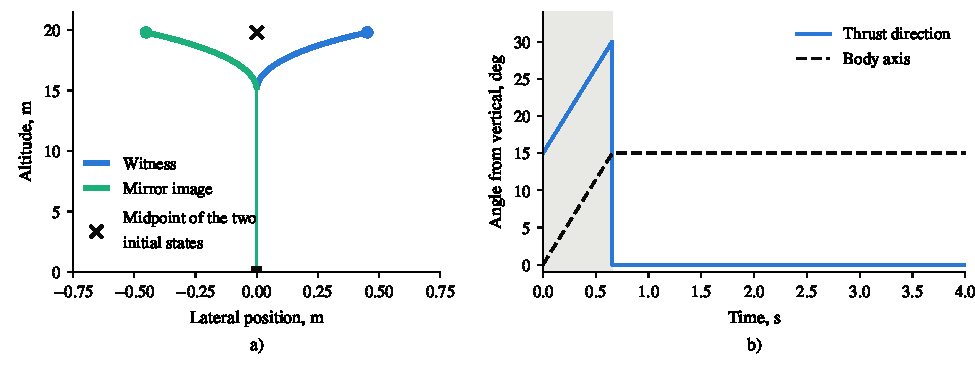
\includegraphics[width=6.5in]{figures/witness.pdf}
\caption{Witnesses of Theorem~\ref{thm:Bstar} for $\Tmin/m_0=5$~m/s$^2$, $\Tmax/m_0=12.5$~m/s$^2$, $\delta=15$~deg,
$\omega=0.4$~rad/s, $s^*=\delta/\omega$, $t_f=4$~s, and constant mass: a)~the two trajectories, with the dive drawn thick and
the lateral scale enlarged; b)~the attitude and thrust direction, with the dive shaded.}\label{fig:witness}
\end{figure}

Figure~\ref{fig:witness} shows the witnesses. With an unlimited rate the body could alternate between the two directions
arbitrarily fast and the midpoint would be landable, which is the 3-DOF situation; with zero rate the thrust could alternate
on the gimbal cone instead. A finite, positive rate limit is what the obstruction needs. The same proof covers upright
touchdown (the body returns to vertical during the brake if $t_f\ge2s^*$), 6-DOF attitude kinematics (the third column of a
rotation matrix with angular velocity bounded by $\omega$ satisfies Eq.~\eqref{eq:AL}), and free final time on a bounded
window, so a search over the final time with a convex program at each value is not lossless either.

\emph{Formal verification.} Theorems~\ref{thm:A} and \ref{thm:Bstar}, both lemmas, and these extensions, with constant
thrust-acceleration bounds and with explicit mass depletion, are formalized in Lean~4 with the Mathlib library
\cite{lean4,mathlib,repo}; the project has no unproved step, and each of the 126 audited declarations depends only on the
three standard axioms. A second reader, working from the manuscript alone, rebuilt the project, wrote an independent
simulator, and searched for a control that lands from $\theta_m$ in the case of Fig.~\ref{fig:witness}; the search came no
closer than 0.020 in the Euclidean norm of $(r_0,v_0)$, whereas it reaches a random landable datum to within $10^{-8}$.
That review also found that an earlier statement of (S1) lacked the bound $\pi/2-\delta$, which the formal statement had
always carried.

\emph{Size of the effect.} Nonconvexity alone does not say how far a complete program must overreach. The proof can be made
quantitative without the equality case: a control whose $W_z$ falls short of $V^*$ by $\eta$ has, by Lemma~\ref{lem:tri}
applied about the body axis at an early instant, nearly the lateral moment of a witness, and tilting during the brake can
cancel that moment only at a cost in $\eta$ that the Cauchy--Schwarz inequality bounds. For $\delta\le\pi/4$ this gives
\begin{equation}\label{eq:eta}
\operatorname{dist}(\theta_m,\F)\ \ge\ \frac{\eta_0}{\sqrt{1+s^{*2}}},\qquad
(1+c_1)\,\eta_0+\sqrt{\tau_{\max}(t_f-s^*)^2\,\eta_0}=\gamma_X:=\frac{5\,\Tmin}{32\,m_0}\sin\delta\,s^{*2},\qquad
c_1=\frac{4\,\tau_{\max}m_0}{\omega\,\Tmin\sin\delta\,s^*} .
\end{equation}
For an 80-kg lander with
thrust between 400 and 1000~N, $\delta=15$~deg, $\omega=0.4$~rad/s, $s^*=\delta/\omega$, and $t_f=7$~s, $\gamma_X=0.087$~m but
$\eta_0=1.3\times10^{-5}$~m: a competitor can cancel the lateral moment of a short dive by tilting slightly during the long
brake. For descents that begin
in the air the gap is therefore proved but small. It grows on short, aggressive maneuvers, as the example of the next
section shows.

\section{The Gimbaled Rigid Body and Its Center of Percussion}\label{sec:model}
The vehicle is a rigid axisymmetric body with mass $m$, transverse inertia $J_t$, and unit body axis $b$.
The engine pivots on the body axis a distance $L$ below the center of mass and delivers the thrust $T=T_ab+T_\perp$, where
$T_\perp\perp b$ is the part produced by deflecting the gimbal. A reaction-control system holds the roll rate at zero, so the
angular velocity $\Omega$ is perpendicular to $b$. With $r$ the position of the center of mass and $\alpha$ the mass flow per
unit thrust, the equations of motion are
\begin{equation}\label{eq:eom}
m\ddot r=T-mg_0\ez,\qquad J_t\dot\Omega=(-Lb)\times T,\qquad \dot b=\Omega\times b,\qquad \dot m=-\alpha\norm T .
\end{equation}
The actuator limits are $\Tmin\le\norm T\le\Tmax$, a gimbal angle $\mu\le\dmax$ with $\tan\mu=\norm{T_\perp}/T_a$, and a tilt
$\angle(b,\ez)\le\thmax<\pi/2$. Table~\ref{tab:vehicle} lists the values used in this paper. In contrast to the model of Sec.~\ref{sec:problem}, the body is now turned by the thrust itself.

\begin{table}[t]\centering
\caption{Vehicle and planning parameters}\label{tab:vehicle}
\small
\begin{tabular}{@{}llll@{}}\toprule
Quantity & Value & Quantity & Value \\\midrule
Wet mass, dry mass & 80 kg, 55.9 kg & Thrust range, physical & 400 to 1000 N \\
Transverse inertia $J_t$ (wet) & 63.6 kg\,m$^2$ & Thrust range, planning & 440 to 920 N \\
Pivot to center of mass $L$ (wet) & 0.589 m & Gimbal limit, physical & $\pm15$ deg per axis, 100 deg/s \\
Center-of-percussion offset $\varepsilon$ & 1.35 m & Gimbal limit, planning $\dmax$ & 10 deg cone \\
Specific impulse & 180 s & Tilt limit $\thmax$ & 20 deg \\\bottomrule
\end{tabular}
\end{table}

Deflecting the gimbal produces the torque that turns the body, but it also pushes the center of mass sideways. One point of the
body is not accelerated by that push. Because $\Omega\perp b$, the lateral part of $\ddot b$ is $\Pib\ddot b=\dot\Omega\times b$
with $\Pib=I-bb^{\mathsf T}$, and the second of Eqs.~\eqref{eq:eom} gives $J_t\,\dot\Omega\times b=-LT_\perp$. Hence
\begin{equation}\label{eq:Tperp}
T_\perp=-m\varepsilon\,\Pib\ddot b,\qquad \varepsilon=\frac{J_t}{mL}.
\end{equation}
Substituting Eq.~\eqref{eq:Tperp} into the first of Eqs.~\eqref{eq:eom} and using $\Pib\ddot b=\ddot b+\norm{\dot b}^2b$ shows
that the point $y=r+\varepsilon b$, the center of percussion, obeys
\begin{equation}\label{eq:cop}
\ddot y=\Bigl(\frac{T_a}{m}-\varepsilon\norm{\dot b}^2\Bigr)b-g_0\ez ,
\end{equation}
provided $\varepsilon$ is constant. The lateral thrust does not appear. Seen from $y$, the gimbaled vehicle is a point mass
whose thrust is locked to the body axis. We assume throughout that $\varepsilon$ is constant along the flight. For constant mass
this holds exactly; with depleting mass it requires $J_t$ to scale with $mL$. The mass-property table of the vehicle's
simulator gives $\varepsilon=1.352$, 1.340, and 1.321~m at 79.9, 75, and 70.4~kg, so the assumption holds to 1\% over a descent.


\subsection{Status of the Impossibility for This Vehicle}
On the gimbaled rigid body the witnesses of Theorem~\ref{thm:Bstar} are not trajectories, because deflecting the thrust
outward rotates the body inward. Equation~\eqref{eq:cop} turns the problem into one with zero gimbal angle and a bounded
angular acceleration for $y$, and with it we proved nonconvexity of the landing set, with upright touchdown at rest and
$r_z\ge0$, at final times of 1, 2, 3, and 5~s by computer-assisted certificates verified in exact arithmetic \cite{repo}. The
certificates assume constant mass and an unlimited gimbal rate, and the certified distances are between $10^{-6}$ and
$10^{-4}$~m. With a gimbal-rate limit and depleting mass the statement rests on numerical evidence. On the model and planning
limits of Table~\ref{tab:vehicle}, a nonconvex solver \cite{ipopt} finds landings 1, 2, and 3~m from the launch point of a
4-s hop launched straight up at 6.3~m/s, but none on the launch point itself, from symmetric initial guesses or from nine
asymmetric ones (Fig.~\ref{fig:ring}): a vehicle rising too fast for the time allowed must shed vertical impulse, with a minimum throttle it can do
so only by tilting, and tilting carries it sideways. The reachable landing points form a ring, so the landable data are not a
convex set. This is evidence, not a proof of infeasibility.

\begin{figure}[t]\centering
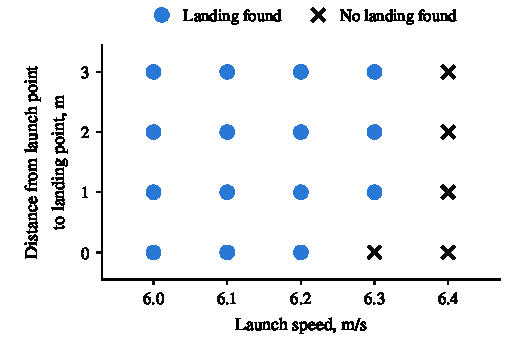
\includegraphics[width=3.4in]{figures/hopring.pdf}
\caption{A 4-s hop of the gimbaled rigid body launched straight up: landing distances at which a nonconvex solver did and did
not find a trajectory.}\label{fig:ring}
\end{figure}

Exactness is therefore out of reach, in proof for the model of Sec.~\ref{sec:problem} and in evidence for this vehicle.
Soundness is not, and Eq.~\eqref{eq:cop} makes it inexpensive.

\section{A Sound Convex Program}\label{sec:program}
\subsection{Flat Map}
Let $y(t)$ be four times continuously differentiable and define $u=\ddot y+g_0\ez$ and $f=\norm u$. Wherever $u\ne0$, let
\begin{equation}\label{eq:flat}
\begin{gathered}
b=\frac uf,\qquad \dot b=\frac{\Pib\dot u}{f},\qquad \Pib\ddot b=\frac{\Pib\ddot u-2\ip b{\dot u}\,\dot b}{f},\qquad
a=f+\varepsilon\norm{\dot b}^2,\qquad \tau=\sqrt{a^2+\varepsilon^2\norm{\Pib\ddot b}^2},\\
m(t)=m_0\exp\Bigl(-\alpha\int_0^t\tau\,\mathrm dt\Bigr),\qquad T_a=ma,\qquad T_\perp=-m\varepsilon\,\Pib\ddot b,\qquad r=y-\varepsilon b .
\end{gathered}
\end{equation}
The attitude, the body rate, the gimbal angle ($\tan\mu=\varepsilon\norm{\Pib\ddot b}/a$), and the throttle ($\norm T=m\tau$) are
algebraic functions of $y$ and its first four derivatives, and the mass is a quadrature. Section~\ref{sec:proof} shows that
Eqs.~\eqref{eq:flat} are the unique solution of Eqs.~\eqref{eq:eom}. Any sufficiently smooth curve $y$ with $u\ne0$ is
therefore a flight of the vehicle, and only the actuator limits remain to be imposed.

\subsection{Spline Parametrization}
The unknown is $y$, a clamped quintic B-spline with $S$ uniform spans of length $h=t_f/S$. It has $S+5$ coefficients per axis,
63 scalars for $S=16$, and it is four times continuously differentiable, so the gimbal angle and the throttle are continuous.
On each span, $u$, $\dot u$, and $\ddot u$ are polynomials of degree 3, 2, and 1. Raising their B\'ezier control points to
degree 3 gives four \emph{control tuples} $(U^j,U_1^j,U_2^j)$, $j=0,\dots,3$, that are linear in the spline coefficients and satisfy
\begin{equation}\label{eq:hull}
(u,\dot u,\ddot u)(t)=\sum_{j=0}^{3}B_j(t)\,(U^j,U_1^j,U_2^j),\qquad B_j(t)\ge0,\qquad \sum_{j=0}^{3}B_j(t)=1,\qquad \int_{\mathrm{span}}B_j\,\mathrm dt=\frac h4 ,
\end{equation}
where $B_j$ are the cubic Bernstein polynomials of the span. Equation~\eqref{eq:hull} is what allows limits to be enforced at
every instant and not only at grid points \cite{vanloock2015}.

\subsection{The Program}
The data are the current position $r_0$, velocity $v_0$, body axis $b_0$, its rate $\dot b_0$, the lateral angular acceleration
$\beta_0=\Pib\ddot b(0)$ that the present gimbal deflection produces, the mass $m_0$, and the time of flight $t_f$; the target is
the origin. Let $p=\ip U\ez$ for a control tuple, $f_0=\ip{b_0}{u(0)}$, and $\Pi_0=I-b_0b_0^{\mathsf T}$. With auxiliary scalars
$q$, $k$, $G$, and $\sigma$ on each tuple and two constants $\phi>0$ and $\ell_b>0$, the program is
\begin{subequations}\label{eq:prog}
\begin{align}
\text{minimize}\quad & \tfrac h4\textstyle\sum\sigma \label{eq:obj}\\
\text{subject to}\quad & y(0)=r_0+\varepsilon b_0,\quad \dot y(0)=v_0+\varepsilon\dot b_0,\quad u(0)=f_0b_0,\quad \Pi_0\dot u(0)=f_0\dot b_0 \notag\\
& \Pi_0\ddot u(0)=f_0\beta_0+2\ip{b_0}{\dot u(0)}\dot b_0 \label{eq:bc0}\\
& y(t_f)=\varepsilon\ez,\quad \dot y(t_f)=0,\quad u_h(t_f)=\dot u_h(t_f)=\ddot u_h(t_f)=0 \label{eq:bcf}\\
& \norm{U_h}\le\tan\thmax\,p,\qquad p\ge\ell_b,\qquad \norm{U_1}^2\le q\,p \label{eq:tilt}\\
& \norm{U_2-k\ez}+\sin\thmax\,|k|+q\le G,\qquad \varepsilon\,G\le\tan\dmax\,(2\phi p-\phi^2) \label{eq:gimbal}\\
& \bigl\|\bigl(\norm U+\varepsilon q/\ell_b,\ \varepsilon G/\ell_b\bigr)\bigr\|\le\sigma \label{eq:sigma}\\
& p\ge\Tmin\,c_s(z_{lo,s}),\qquad \sigma\le\Tmax\,\tau_s(z_{up,s}) \label{eq:mass}
\end{align}
\end{subequations}
where the subscript $h$ denotes the horizontal part of a vector, Eqs.~(\ref{eq:tilt}--\ref{eq:mass}) hold on every control
tuple, and $s$ indexes spans. The quantities in Eq.~\eqref{eq:mass} bracket the logarithm of the mass:
\begin{equation}\label{eq:z}
z_{up,s}=\ln m_0-\alpha\bigl(\dot y_z(t_s)-\dot y_z(0)+g_0t_s\bigr),\qquad z_{lo,s}=\ln m_0-\alpha\,\tfrac h4\!\!\sum_{\text{spans}\le s}\sum_{j}\sigma^j ,
\end{equation}
with $t_s$ the start of span $s$. Both are affine in the unknowns. The function $c_s$ is the chord of $e^{-z}$ on an interval
to which $z_{lo,s}$ is confined by two further linear constraints, and $\tau_s$ is a tangent of $e^{-z}$; the dry-mass limit is
$z_{lo,S}\ge\ln m_{dry}$. Every constraint is linear or a second-order cone, so Eqs.~\eqref{eq:prog} form an SOCP. The boundary
conditions are linear because $f_0$ and $\ip{b_0}{\dot u(0)}$ are linear in the coefficients, and $(r_0,v_0)$ enter affinely,
exactly as in LCvx.

The reading of the constraints is as follows. Equations~\eqref{eq:bc0} start the plan at the present position, velocity,
attitude, body rate, and gimbal deflection. Equations~\eqref{eq:bcf} end it at rest on the target, upright, without rotation,
and with the gimbal centered. The first of Eqs.~\eqref{eq:tilt} is the tilt limit, and it is exact. The second of
Eqs.~\eqref{eq:gimbal} is the gimbal limit: the snap and the squared jerk of the center-of-percussion path are bounded by the
authority of the gimbal. Equations~\eqref{eq:sigma} and \eqref{eq:mass} are the throttle limits, with the vertical part of $u$
standing in for its magnitude in the lower one. The altitude floor and a glide slope on $r$ are added at sampled instants with
a slack variable, as is usual. The constants are $\phi=7.5$~m/s$^2$, the specific force at which the gimbal constraint is
tightest, and $\ell_b=\Tmin/m_0$. Any positive values keep the guarantee of Sec.~\ref{sec:proof}; they change only how much of
the feasible set is retained.

\section{Soundness}\label{sec:proof}
\begin{theorem}\label{thm:sound}
Assume $\varepsilon$ is constant and $\angle(b_0,\ez)\le\thmax$, and let $y$ be feasible for Eqs.~\eqref{eq:prog}. Then
Eqs.~\eqref{eq:eom}, started from $(r_0,v_0,b_0,\dot b_0,m_0)$ and driven by the thrust $T=T_ab+T_\perp$ of
Eqs.~\eqref{eq:flat}, have the unique solution $r=y-\varepsilon b$, and this solution 1) begins with the lateral thrust the
gimbal is producing, $T_\perp(0)=-m_0\varepsilon\beta_0$; 2) ends with $r=\dot r=0$, $b=\ez$, $\dot b=0$, and $T_\perp=0$;
3) satisfies $\Tmin\le\norm T\le\Tmax$, $\mu\le\dmax$, and $\angle(b,\ez)\le\thmax$ at every $t\in[0,t_f]$; and
4) consumes at most $m_0[1-\exp(-\alpha\tfrac h4\sum\sigma)]$ of propellant.
\end{theorem}
\begin{proof}
\emph{Step 1: the flat map solves the equations of motion.} Differentiating $u=fb$ twice and projecting with $\Pib$ gives
$\Pib\dot u=f\dot b$ and $f\,\Pib\ddot b=\Pib\ddot u-2\dot f\dot b$ with $\dot f=\ip b{\dot u}$, so the quantities named $\dot b$
and $\Pib\ddot b$ in Eqs.~\eqref{eq:flat} are the derivatives of $b$. Take $\Omega=b\times\dot b$. Then $\Omega\perp b$,
$\Omega\times b=\dot b$, and $\dot\Omega=b\times\Pib\ddot b$. The torque of the thrust is $(-Lb)\times T=Lm\varepsilon\,b\times\Pib\ddot b
=J_t\dot\Omega$, because $m\varepsilon L=J_t$. The force is $T-mg_0\ez=m(f+\varepsilon\norm{\dot b}^2)b-m\varepsilon(\ddot b+\norm{\dot b}^2b)-mg_0\ez
=m(\ddot y-\varepsilon\ddot b)=m\ddot r$. Finally $\norm T=m\tau$ and $\dot m=-\alpha\tau m$ by the definition of $m$. The right-hand
sides of Eqs.~\eqref{eq:eom} are locally Lipschitz in the state, so the solution is unique.

\emph{Step 2: boundary conditions.} The end control points of a B\'ezier polygon are values of the curve, so $u_z\ge\ell_b>0$ at
$t=0$ and $t=t_f$. At $t=0$, $u(0)=f_0b_0$ with positive vertical components forces $f_0>0$ and $b(0)=b_0$; the next two
conditions of Eq.~\eqref{eq:bc0} then give $\dot b(0)=\dot b_0$ and $\Pib\ddot b(0)=\beta_0$ by Step~1, and the first two give
$r(0)=r_0$ and $\dot r(0)=v_0$. At $t_f$, $u_h=0$ gives $b=\ez$, then $\dot u_h=0$ gives $\dot b=0$, then $\ddot u_h=0$ gives
$\Pib\ddot b=0$, and $r=y-\varepsilon\ez=0$, $\dot r=\dot y=0$.

\emph{Step 3: pointwise bounds.} Fix an instant and suppose that numbers $q$, $k$, $G$, $\sigma$ satisfy
Eqs.~(\ref{eq:tilt}--\ref{eq:sigma}) with $(U,U_1,U_2)$ replaced by $(u,\dot u,\ddot u)$. Let $p=u_z\le f$. The first of
Eqs.~\eqref{eq:tilt} is $\tan\angle(b,\ez)\le\tan\thmax$. Next, $f\norm{\dot b}^2=\norm{\Pib\dot u}^2/f\le\norm{\dot u}^2/p\le q$.
For the angular acceleration, $f\,\Pib\ddot b=\Pib(\ddot u-k\ez)+k\,\Pib\ez-2\ip b{\dot u}\Pib\dot u/f$. The norm of the first term is at
most $\norm{\ddot u-k\ez}$; $\norm{\Pib\ez}=\sin\angle(b,\ez)\le\sin\thmax$; and
$2|\ip b{\dot u}|\norm{\Pib\dot u}\le\norm{\dot u}^2$ because the two factors are the parts of $\dot u$ along and across $b$. Hence
$f\norm{\Pib\ddot b}\le G$. Since $f^2\ge p^2\ge2\phi p-\phi^2$, the second of Eqs.~\eqref{eq:gimbal} gives
$\varepsilon\norm{\Pib\ddot b}\le\tan\dmax f\le\tan\dmax\,a$, which is $\mu\le\dmax$. Lastly $p\le f\le a\le\tau$, and
$a\le\norm u+\varepsilon q/\ell_b$ and $\varepsilon\norm{\Pib\ddot b}\le\varepsilon G/\ell_b$ because $f\ge p\ge\ell_b$, so
$p\le\tau\le\sigma$ by Eq.~\eqref{eq:sigma}.

\emph{Step 4: every instant.} Equations~(\ref{eq:tilt}--\ref{eq:sigma}) describe a convex set of points $(U,U_1,U_2,q,k,G,\sigma)$
that is the same for the four control tuples of a span. By Eq.~\eqref{eq:hull}, $(u,\dot u,\ddot u)(t)$ together with the
Bernstein-weighted auxiliary numbers is a convex combination of four points of that set, so it lies in the set. Step~3
therefore applies at every instant, with $\sigma(t)=\sum_jB_j(t)\sigma^j$.

\emph{Step 5: mass.} Let $z=\ln m$, so that $\dot z=-\alpha\tau$ and $p\le\tau\le\sigma(t)$. On span $s$,
$z(t)\le z(t_s)\le\ln m_0-\alpha\int_0^{t_s}u_z\,\mathrm dt=z_{up,s}$ and $z(t)\ge z(t_{s+1})\ge\ln m_0-\alpha\int_0^{t_{s+1}}\sigma\,\mathrm dt=z_{lo,s}$,
using the last of Eqs.~\eqref{eq:hull}. Because $e^{-z}$ is decreasing and convex, a chord lies above it and a tangent below it,
so Eq.~\eqref{eq:mass} gives $p(t)\ge\Tmin e^{-z(t)}$ and $\sigma(t)\le\Tmax e^{-z(t)}$, that is,
$\Tmin\le mp\le m\tau=\norm T\le m\sigma\le\Tmax$. The fuel bound is $z(t_f)\ge z_{lo,S}$.
\end{proof}

No relaxation is used, so there is no tightness to establish; this is the difference from LCvx. The price is stated next.

\begin{proposition}\label{prop:inc}
For fixed $b_0$, $\dot b_0$, $\beta_0$, $m_0$, and $t_f$, the set of $(r_0,v_0)$ at which Eqs.~\eqref{eq:prog} are feasible is
convex and is contained in $F$. Whenever $F$ is not convex, the containment is strict.
\end{proposition}
\begin{proof}
The data enter only the right-hand sides of the first two conditions of Eq.~\eqref{eq:bc0}, so the projection argument of
Theorem~\ref{thm:A} gives convexity. Containment is Theorem~\ref{thm:sound}. A convex set cannot equal a nonconvex one.
\end{proof}

The program must therefore refuse some landings that exist. The loss has three sources: the lower throttle limit is imposed on
the vertical part of the thrust, so the program never plans to shed thrust by tilting, which is the maneuver the obstruction of
Sec.~\ref{sec:dive} is built from; the interaction of throttle changes with rotation is bounded, not computed; and control
polygons contain the curves they bound. Section~\ref{sec:results} measures the size of the loss. Two limits are outside the
theorem. The gimbal and throttle slew rates depend on the fifth derivative of $y$ and are not constrained by
Eqs.~\eqref{eq:prog}; they are evaluated exactly on every plan, and a plan that violates them is not flown. The altitude and
glide-slope constraints hold at the sampled instants only.


\section{Guidance Algorithm and Results}\label{sec:results}
\subsection{Algorithm}\label{sec:algorithm}
The guidance law has three steps. 1) Once, before the descent, the time of flight is set to the smallest $t_f$ at which
Eqs.~\eqref{eq:prog} are feasible, found by bisection in about ten solves, plus a margin of 0.25~s. 2) At every guidance step
the program is solved for the remaining time of flight from the current state estimate; nothing is carried over from the
previous plan, and no initial trajectory, trust region, or penalty weight is required. 3) At every control step the reference
position, velocity, attitude, body rate, throttle, and gimbal angle are evaluated from Eqs.~\eqref{eq:flat} in closed form
and passed to the tracking controller. If a solve is infeasible or its plan fails the slew-rate check, the flight time is
extended by up to 1~s, and otherwise the previous plan, which remains valid, is kept. For $S=16$ the program has 63 spline
coefficients; as passed to the solver it has about 1000 variables and 480 second-order cones, of the types used by 3-DOF
LCvx, and one solve takes about 40~ms.

\subsection{Setup}
All results are numerical and use the vehicle of Table~\ref{tab:vehicle}. The baseline, denoted S, is a standard 6-DOF SCvx
implementation \cite{mao2016,szmuk2018} on the quaternion rigid body with 35 intervals, virtual control, and a trust region,
with the same planning limits. The program of Eqs.~\eqref{eq:prog} is denoted F. Both use the Clarabel interior-point solver
on a four-core desktop processor. The simulated plant is the quaternion rigid body with mass-dependent inertia and lever arm,
a $\pm15$~deg gimbal box with a 100~deg/s slew limit, a 400 to 1000~N throttle with a 2000~N/s slew limit, wind of up to
3~m/s with gusts, 2\% thrust noise, a 5\% error in specific impulse, and gimbal misalignment. One tracking controller, a
linear-quadratic regulator in center-of-percussion coordinates at 50~Hz, serves both planners. The test set is 40 in-air
descents (altitude 40 to 60~m, offset up to 21~m, initial tilt up to 3~deg) and 30 hops launched from the pad at 5 to 6~m/s
toward a point up to 4~m away. A landing succeeds if the touchdown speed is at most 1~m/s, the lateral error at most 1~m,
and the tilt at most 5~deg.

\subsection{Single Plans: Cost, Exactness, and Soundness}
On eight in-air scenarios at equal final time, F uses 0.10\% more fuel than S on average and 0.28\% at most, with one SOCP
and a median solver time of 0.046~s against 25 to 35 SOCPs and 1.30~s. Its minimum feasible final time is 0.04 to 0.22~s
longer, and up to 0.41~s longer on 4-s hops; this is the incompleteness of Proposition~\ref{prop:inc}. To test Step~1 of the
proof, the throttle and gimbal commands of F were applied without feedback to the quaternion rigid body with depleting mass
and constant $\varepsilon$, integrated to a relative tolerance of $10^{-13}$: in 16 replays the vehicle came to rest within
23~nm of the target, which is integration error. To test Theorem~\ref{thm:sound}, 300 random problems were each solved with
the constants above and with randomly chosen ones; 458 of the 600 solves were feasible, and no plan violated a planning limit
at any of 1201 instants. To test Proposition~\ref{prop:inc}, both planners and a nonconvex solver were run on 20 hops of
exactly 4~s. No flyable plan was found for 11 of the targets, and F is infeasible at all 11; it is also infeasible at five of
the nine targets where a plan exists. A 3-DOF LCvx program reports an optimal solution at all 20, which is the false
feasibility that Theorem~\ref{thm:A} predicts for a complete program.

\subsection{Closed Loop with Computation Time Counted}
Simulation studies of guidance commonly apply each plan at the instant its state was sampled. Here a plan computed from the
state at time $t$ becomes active at $t$ plus its solver time, and each planner replans as soon as it can: S at most every
0.5~s and F every 0.1~s. Table~\ref{tab:closed} and Fig.~\ref{fig:td} give the results. Both planners land every case. F is more accurate
laterally by more than an order of magnitude, touches down more slowly, and moves the gimbal a third as far. On hops it uses
5\% more fuel, because it flies them slightly longer. With every solver time multiplied by four, to represent a slower flight
computer, S fails four of the 30 hops, and F, replanning every 0.2~s, fails none. The source of the advantage should be
stated carefully: when both planners replan at 1~Hz, plans are applied instantly, and both fly the same final time, the
lateral accuracy is the same (medians of 3.1~cm in the air and 2.4~cm on hops for each). The accuracy in
Table~\ref{tab:closed} comes from the replanning rate, which a solver time of 30~ms permits and a solver time of 1~s does not.

\begin{table}[t]\centering
\caption{Closed-loop results with each plan applied after its solver time (median / 95th percentile / maximum)}\label{tab:closed}
\small\setlength{\tabcolsep}{4.5pt}
\begin{tabular}{@{}lcccc@{}}\toprule
 & \multicolumn{2}{c}{In-air descents (40 runs)} & \multicolumn{2}{c}{Pad hops (30 runs)} \\\cmidrule(lr){2-3}\cmidrule(l){4-5}
 & S & F & S & F \\\midrule
Successful landings & 40 & 40 & 30 & 30 \\
Lateral error, cm & 5.9 / 15.7 / 18.3 & 0.2 / 0.8 / 1.1 & 3.9 / 7.6 / 8.2 & 0.4 / 1.4 / 2.0 \\
Touchdown speed, m/s & 0.23 / 0.46 / 0.58 & 0.19 / 0.28 / 0.29 & 0.54 / 0.81 / 0.88 & 0.14 / 0.22 / 0.23 \\
Tilt at touchdown, deg & 0.21 / 0.70 / 1.23 & 0.11 / 0.30 / 0.63 & 0.96 / 2.46 / 2.54 & 0.20 / 0.62 / 0.87 \\
Fuel, mean, kg & 3.58 & 3.52 & 1.46 & 1.54 \\
Solver time per replan, s (mean / maximum) & 1.05 / 4.9 & 0.031 / 0.39 & 0.35 / 2.4 & 0.017 / 0.052 \\
Convex programs per plan, mean & 20.2 & 1.4 & 12.7 & 1.1 \\
Gimbal travel per flight, mean, deg & 156 & 45 & 182 & 62 \\\bottomrule
\end{tabular}
\end{table}

\begin{figure}[t]\centering
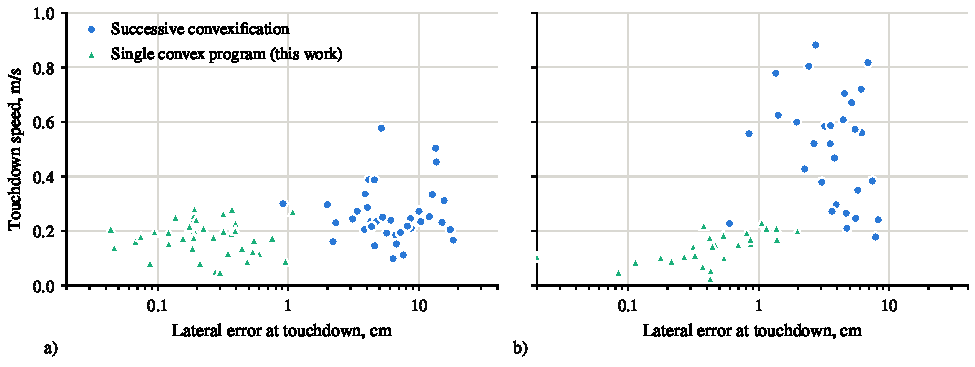
\includegraphics[width=\linewidth]{figures/touchdown.pdf}
\caption{Touchdown accuracy with computation time counted: a) 40 in-air descents and b) 30 pad hops.}\label{fig:td}
\end{figure}

\subsection{Limitations}
F is worse than S in fuel on short hops and in minimum flight time. The slew-rate limits are outside
Theorem~\ref{thm:sound}; fewer than 1\% of replans failed the check and were not flown. Theorem~\ref{thm:sound} is proved here
and tested numerically but is not machine-checked, apart from Eq.~\eqref{eq:cop} for constant mass, and it has not had an
independent reader as Theorem~\ref{thm:Bstar} has. The assumption of constant $\varepsilon$ must be confirmed from measured mass
properties. Nothing here has been run on flight hardware, with actuator lag, or with state-estimation error, and the SCvx
baseline was not retuned for speed. On the impossibility side, the proved gap is small for descents that begin in the air, and
for the gimbaled rigid body the result is certified only at four final times under simplifying assumptions.

\section{Conclusion}
For powered descent with a finite-rate attitude, a single convex program of the kind lossless convexification belongs to
cannot be exact: an exact program would make the set of landable initial states convex, and a dive to one side followed by a
brake, together with its mirror image, shows that the set is not convex at any final time. This is machine-checked. What a
single convex program can still be is sound. For a lander steered by one gimbaled engine, writing the problem for the center
of percussion removes the coupling between steering and translation and leaves the actuator limits as the only nonconvex
part; restricting those limits, instead of relaxing them, yields one second-order cone program whose plans are flyable at
every instant by proof. It costs a tenth of a percent of fuel and a few tenths of a second of minimum flight time, has no
initial guess, trust region, or iteration count, and solves fast enough to replan at the rate of the control system, which in
our simulations mattered more for touchdown accuracy than the last fraction of a percent of optimality. Future work is a
certificate of nonconvexity that accounts for the gimbal-rate limit and depleting mass, an independent check and
formalization of the soundness proof, slew-rate limits inside the guarantee, and flight.

\section*{Acknowledgments}
% AIAA policy (Ethical Standards, Sec. 3) requires a description of AI use here and a disclosure at submission.
% The first two sentences below are a factual description of how this work was produced. Complete the rest truthfully.
An artificial-intelligence system (Claude, Anthropic) was used extensively in this work. It derived and wrote the proofs,
wrote the Lean formalization and the planning and simulation software, ran the numerical experiments, and drafted the text
and figures of this manuscript. [State here what the Contributing Student Authors did themselves, for example: posed the
question, defined the vehicle data, directed the investigation, and checked the derivations, the code, and the results.] The
independent check of the impossibility proof was carried out by [name of the reviewer, with permission]. [State any other
contributors and sponsors.] The authors are responsible for the content of the paper.

\begin{thebibliography}{99}
\bibitem{acikmese2007} A\c{c}{\i}kme\c{s}e, B., and Ploen, S. R., ``Convex Programming Approach to Powered Descent Guidance for Mars
Landing,'' \emph{Journal of Guidance, Control, and Dynamics}, Vol.~30, No.~5, 2007, pp.~1353--1366. \url{https://doi.org/10.2514/1.27553}.
\bibitem{acikmese2011} A\c{c}{\i}kme\c{s}e, B., and Blackmore, L., ``Lossless Convexification of a Class of Optimal Control Problems
with Non-Convex Control Constraints,'' \emph{Automatica}, Vol.~47, No.~2, 2011, pp.~341--347. \url{https://doi.org/10.1016/j.automatica.2010.10.037}.
\bibitem{acikmese2013} A\c{c}{\i}kme\c{s}e, B., Carson, J. M., and Blackmore, L., ``Lossless Convexification of Nonconvex Control Bound
and Pointing Constraints of the Soft Landing Optimal Control Problem,'' \emph{IEEE Transactions on Control Systems Technology},
Vol.~21, No.~6, 2013, pp.~2104--2113. \url{https://doi.org/10.1109/TCST.2012.2237346}.
\bibitem{malyuta2022} Malyuta, D., Reynolds, T. P., Szmuk, M., Lew, T., Bonalli, R., Pavone, M., and A\c{c}{\i}kme\c{s}e, B., ``Convex
Optimization for Trajectory Generation: A Tutorial on Generating Dynamically Feasible Trajectories Reliably and Efficiently,''
\emph{IEEE Control Systems Magazine}, Vol.~42, No.~5, 2022, pp.~40--113. \url{https://doi.org/10.1109/MCS.2022.3187542}.
\bibitem{mao2016} Mao, Y., Szmuk, M., and A\c{c}{\i}kme\c{s}e, B., ``Successive Convexification of Non-Convex Optimal Control Problems
and Its Convergence Properties,'' \emph{2016 IEEE 55th Conference on Decision and Control}, IEEE, 2016, pp.~3636--3641.
\url{https://doi.org/10.1109/CDC.2016.7798816}.
\bibitem{szmuk2018} Szmuk, M., and A\c{c}{\i}kme\c{s}e, B., ``Successive Convexification for 6-DoF Mars Rocket Powered Landing with
Free-Final-Time,'' AIAA Paper 2018-0617, Jan. 2018. \url{https://doi.org/10.2514/6.2018-0617}.
\bibitem{szmuk2020} Szmuk, M., Reynolds, T. P., and A\c{c}{\i}kme\c{s}e, B., ``Successive Convexification for Real-Time
Six-Degree-of-Freedom Powered Descent Guidance with State-Triggered Constraints,'' \emph{Journal of Guidance, Control, and
Dynamics}, Vol.~43, No.~8, 2020, pp.~1399--1413. \url{https://doi.org/10.2514/1.G004549}.
\bibitem{fliess1995} Fliess, M., L\'evine, J., Martin, P., and Rouchon, P., ``Flatness and Defect of Non-Linear Systems: Introductory
Theory and Examples,'' \emph{International Journal of Control}, Vol.~61, No.~6, 1995, pp.~1327--1361. \url{https://doi.org/10.1080/00207179508921959}.
\bibitem{martin1996} Martin, P., Devasia, S., and Paden, B., ``A Different Look at Output Tracking: Control of a VTOL Aircraft,''
\emph{Automatica}, Vol.~32, No.~1, 1996, pp.~101--107. \url{https://doi.org/10.1016/0005-1098(95)00099-2}.
\bibitem{mellinger2011} Mellinger, D., and Kumar, V., ``Minimum Snap Trajectory Generation and Control for Quadrotors,''
\emph{2011 IEEE International Conference on Robotics and Automation}, IEEE, 2011, pp.~2520--2525. \url{https://doi.org/10.1109/ICRA.2011.5980409}.
\bibitem{desiderio2013} Desiderio, D., and Lovera, M., ``Guidance and Control for Planetary Landing: Flatness-Based Approach,''
\emph{IEEE Transactions on Control Systems Technology}, Vol.~21, No.~4, 2013, pp.~1280--1294. \url{https://doi.org/10.1109/TCST.2012.2202664}.
\bibitem{vanloock2015} Van Loock, W., Pipeleers, G., and Swevers, J., ``Optimal Motion Planning for Differentially Flat Systems with
Guaranteed Constraint Satisfaction,'' \emph{2015 American Control Conference}, IEEE, 2015, pp.~4245--4250. \url{https://doi.org/10.1109/ACC.2015.7171996}.
\bibitem{wang2026} Wang, C., and Chen, Z., ``B-Spline-Based Convex Programming for Fuel-Optimal Powered Descent Guidance,''
\emph{Advances in Space Research}, Vol.~78, No.~4, 2026, pp.~3919--3934. \url{https://doi.org/10.1016/j.asr.2026.06.014}.
\bibitem{repo} Propulsive Landers at Georgia Tech, ``lossless-navigation-paper: Lean Proofs, Certificates, and Guidance Software for
Powered Descent,'' software and data repository, 2026. \url{https://github.com/Propulsive-Landers-GT/lossless-navigation-paper}.
\bibitem{aumann1965} Aumann, R. J., ``Integrals of Set-Valued Functions,'' \emph{Journal of Mathematical Analysis and Applications},
Vol.~12, No.~1, 1965, pp.~1--12. \url{https://doi.org/10.1016/0022-247X(65)90049-1}.
\bibitem{lean4} de Moura, L., and Ullrich, S., ``The Lean 4 Theorem Prover and Programming Language,'' \emph{Automated Deduction --
CADE 28}, Lecture Notes in Computer Science, Vol.~12699, Springer, Cham, 2021, pp.~625--635. \url{https://doi.org/10.1007/978-3-030-79876-5_37}.
\bibitem{mathlib} The mathlib Community, ``The Lean Mathematical Library,'' \emph{Proceedings of the 9th ACM SIGPLAN International
Conference on Certified Programs and Proofs}, ACM, New York, 2020, pp.~367--381. \url{https://doi.org/10.1145/3372885.3373824}.
\bibitem{ipopt} W\"achter, A., and Biegler, L. T., ``On the Implementation of an Interior-Point Filter Line-Search Algorithm for
Large-Scale Nonlinear Programming,'' \emph{Mathematical Programming}, Vol.~106, No.~1, 2006, pp.~25--57. \url{https://doi.org/10.1007/s10107-004-0559-y}.
\end{thebibliography}
\end{document}
